SocratiCode expone un panel de administración a través de Django Admin, accesible únicamente para usuarios con permisos de administrador. Desde este panel es posible gestionar los datos de la aplicación y, en particular, ajustar la configuración global del sistema sin necesidad de modificar el código ni reiniciar el servidor.

La sección de Configuración del sistema, visible en la \autoref{fig:admin-panel}, permite controlar el comportamiento del moderador de contenido. El administrador puede activar o desactivar la moderación de entrada, la de salida, ambas a la vez o ninguna de las dos. También es posible ajustar el umbral de palabras que determina con qué frecuencia se evalúa la salida del tutor durante la generación.

\begin{figure}[Panel de administración]{fig:admin-panel}{Panel de administración de SocratiCode con la sección de configuración del sistema.}
    \centering
    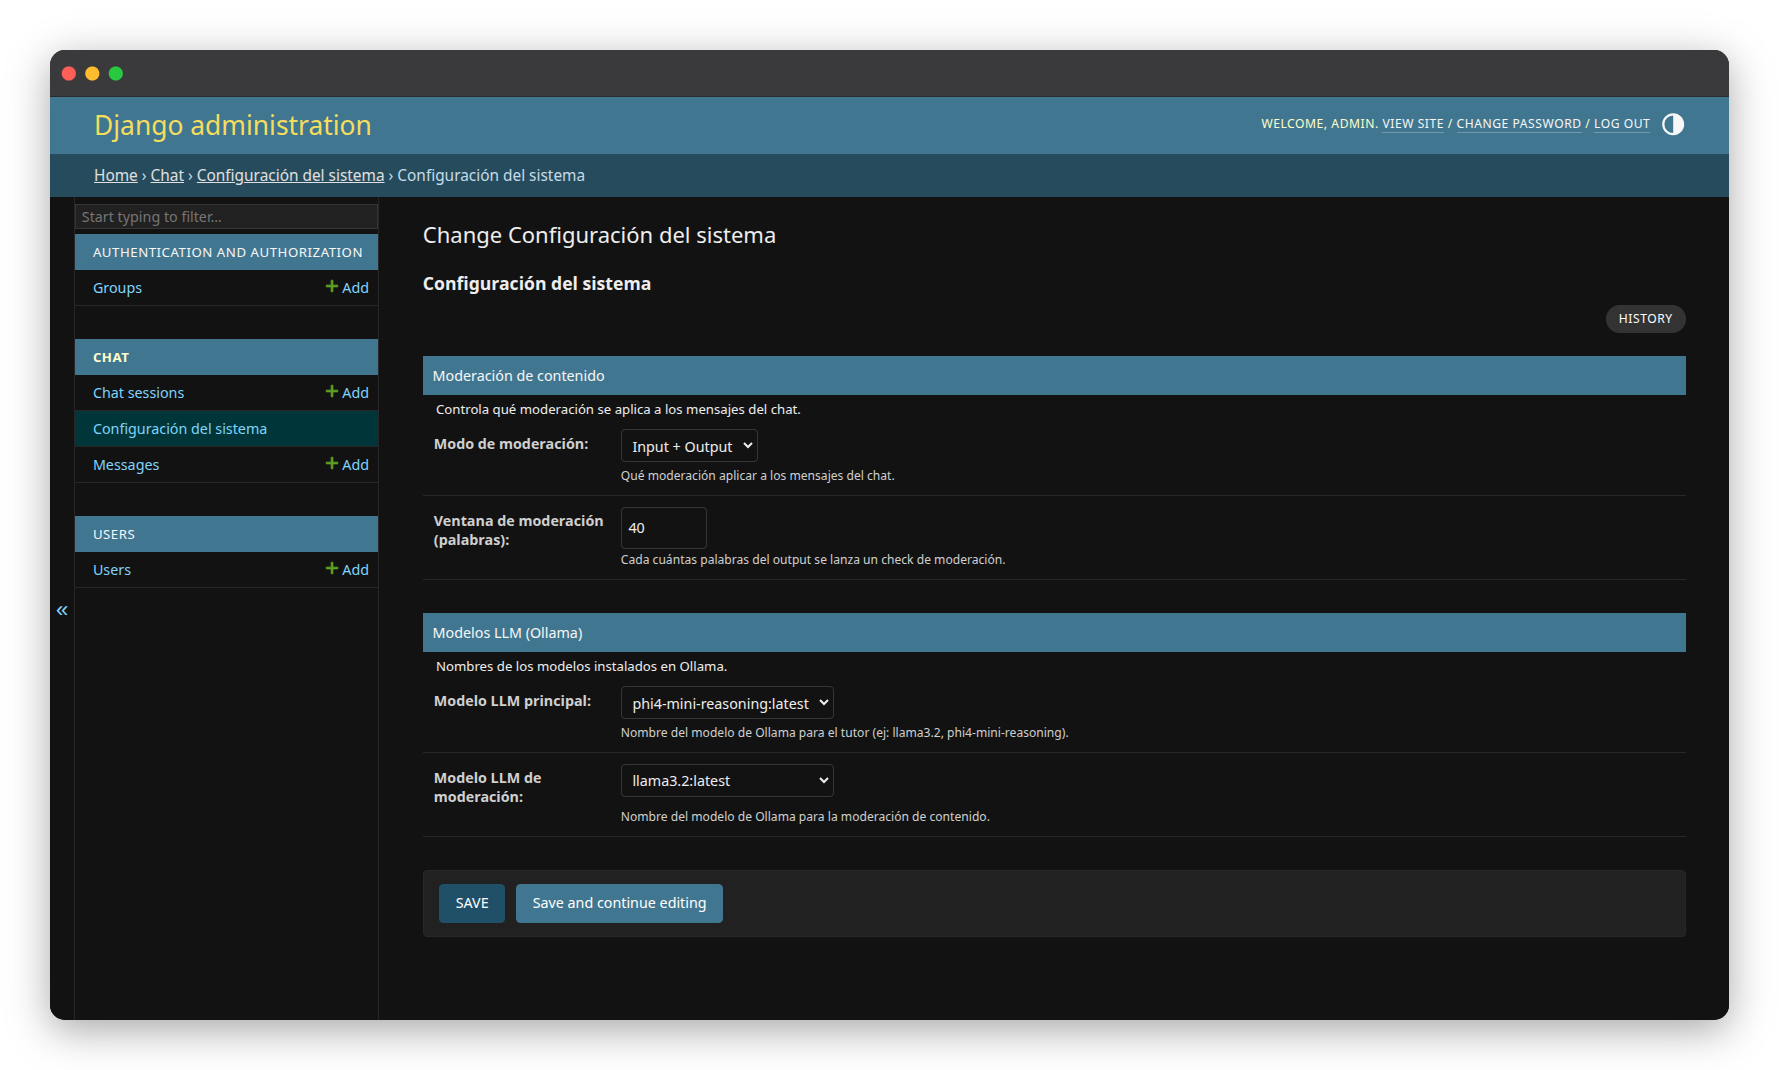
\includegraphics[width=\textwidth]{./pantallas/pantalla_admin.png}
\end{figure}
